% !TEX program = xelatex
\documentclass[11pt,a4paper,UTF8]{ctexart}

\usepackage{syntonly}
%\syntaxonly %不生成DVI或PDF,用来快速编译排查错误。
\usepackage[colorlinks=true]{hyperref}
\usepackage[backend=bibtex]{biblatex}
\usepackage[top=0.7in,bottom=0.7in,left=0.7in,right=0.7in]{geometry}
\usepackage{xeCJK}
\setCJKmainfont[BoldFont = STZhongsong, ItalicFont = STKaiti]{STSong}
\usepackage{graphicx}
%\graphicspath{images/}
\ctexset {section = {format={\Large\bfseries}}}

    \title{\textbf{如何利用一张图像来生成多张纹理贴图}\\ \emph{\small{\CJKfontspec[FakeSlant = 0.2]{STSong}(用8个步骤)}}}
    \author{翻译by Mr. Kin\\ 译者博客:https://kin-sir.github.io \\译者E-mail:1355093365@qq.com \\译文PDF\href{https://pan.baidu.com/s/14aZk-tkii_cgBtUj9LVtoQ}{下载地址},提取码:bqt7 }
    \date{修改于2019.4.26}

\begin{document}
\maketitle

\noindent \emph{\CJKfontspec[FakeSlant = 0.2]{STSong}译者的话:该篇文章实现的思路并不全然是对的,这从原作者发表文章的网站的评论中可以看出,不少网友指出其中的一些不妥之处,各位看官都可以访问\href{http://www.reynantemartinez.com/how-to-generate-texture-maps-from-a-single-image}{文章链接}来观看这些评论。之所以还选择翻译这篇文章,是因为挺欣赏这篇教程背后的思想 - 利用Blender从单个纹理图片生成多张纹理贴图。这篇教程如果能修正错误内容的话,相信会是一篇很优秀的文章。四年前的文章,懒得追溯了,望各位看官能从中有所收获,并借鉴其它一些资料来制作出属于自己的纹理贴图。}

\noindent \rule[5pt]{500pt}{.5pt}

大多时候,逼真的表面和渲染会要求你使用许多类型的贴图,例如\underline{漫反射}(Diffuse),\underline{高光}(Specular),\underline{置换}(Displacement),\underline{粗糙度}(Roughness)等。但是,如果你没有专业的软件,如CrazyBump,Knald,Bitmap2Material或者类似的,那么贴图对你来说是一个大问题了。

在这个简短的教程里,我会给你展示如何利用一张纹理图像和Blender的Cycles材质节点来生成多张通用的纹理贴图。不过,在这里展示的技巧也是适用于其它软件。

本教程结束之时,在关于如何使用各类节点技巧来熟练地操作纹理贴图的方面上,你应该能对其有个基本的理解。

\noindent \rule[-.4pt]{500pt}{.5pt}

\noindent {\large\textbf{可供选择的下载}}
\begin{itemize}
    \item \href{http://www.weebly.com/uploads/4/7/3/9/4739042/texture_map_generator-starter_file_by_reynante_martinez.blend}{starter.blend 文件}
    \item \href{http://www.weebly.com/uploads/4/7/3/9/4739042/texture_map_generator-finished_file_by_reynante_martinez.blend}{finished.blend 文件}
    \item \href{http://cgtextures.com/texview.php?id=12892&PHPSESSID=seph6oah7l4b965vnhm4qam9r5}{木板纹理}(外部链接)
\end{itemize}

\noindent {\large\textbf{可获取的格式}}
\begin{itemize}
    \item \href{http://www.reynantemartinez.com/how-to-generate-texture-maps-from-a-single-image}{网站文章}
    \item Youtube 视频(即将来临)
\end{itemize}

\noindent {\large\textbf{使用的软件}}
\begin{itemize}
   \item \href{http://blender.org/}{Blender 2.74}
   \item Cycles
\end{itemize}

准备好了?让我们开始吧!

\newpage
\section{基本的材质设置}
开始时,准备一个简单的\underline{漫反射}(Diffuse)和\underline{光泽}(Glossy)混合材质并使用一个\underline{图像纹理}(Image Texture)节点作为漫反射的输入。此刻的效果并不是很好,但我们会在下一步中提升它。

\begin{figure}[hb]
    \centering
    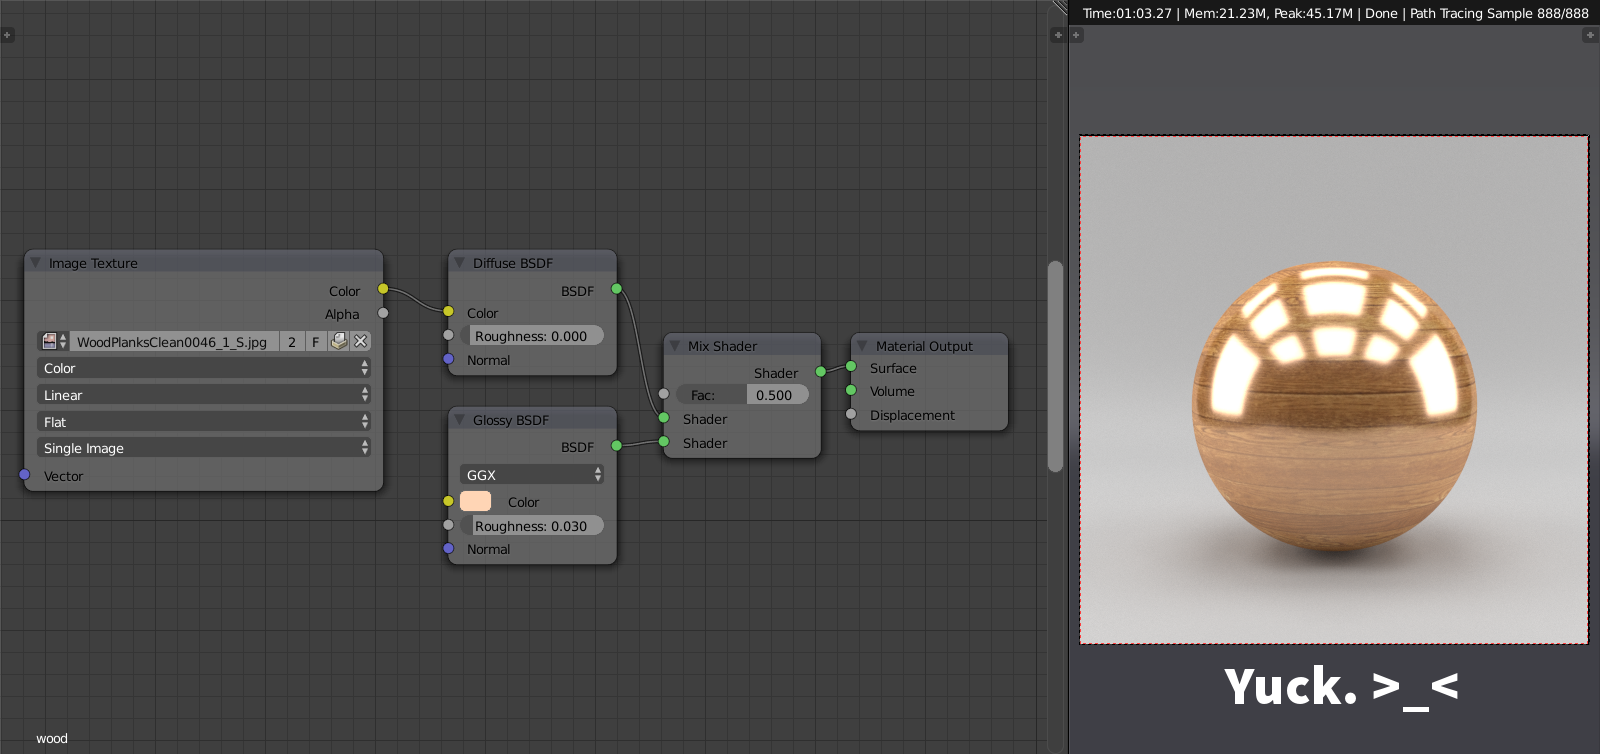
\includegraphics[scale=0.41]{step1}
\end{figure}

\section{创建\underline{漫反射梯度}(Diffuse Gradient)}
这一步完全是可选择性做的,但这一步能使\underline{着色器}(shader)增加一点真实感,至少对我个人来说是这样。:)

在\underline{漫反射着色器}(Diffuse shader)上创建梯度效果,需要使用\textbf{\underline{RBG 曲线}(RGB Curves)}\emph{(Add>Color\\>RGB Curves)}节点来使基色变暗,而且还需使用\textbf{\underline{混合}(Mix)}\emph{(Add>Color>MixRGB)}\footnote{此处原文为\textbf{Mix}\emph{(Add>Shader>Mix Shader)},依照图片看,有误,译文已更正为MixRGB。}节点来混合RGB曲线节点和图像纹理节点\footnote{此处原文为the original diffuse node,本意指初始的图像纹理输入节点,因怕读者误解,译文直接点明Image Texture,不按原意翻译。},并添加\textbf{\underline{层权重}(Layer Weight)}\emph{(Add>Input>Layer Weight)}节点作为系数。

\begin{figure}[hb]
    \centering
    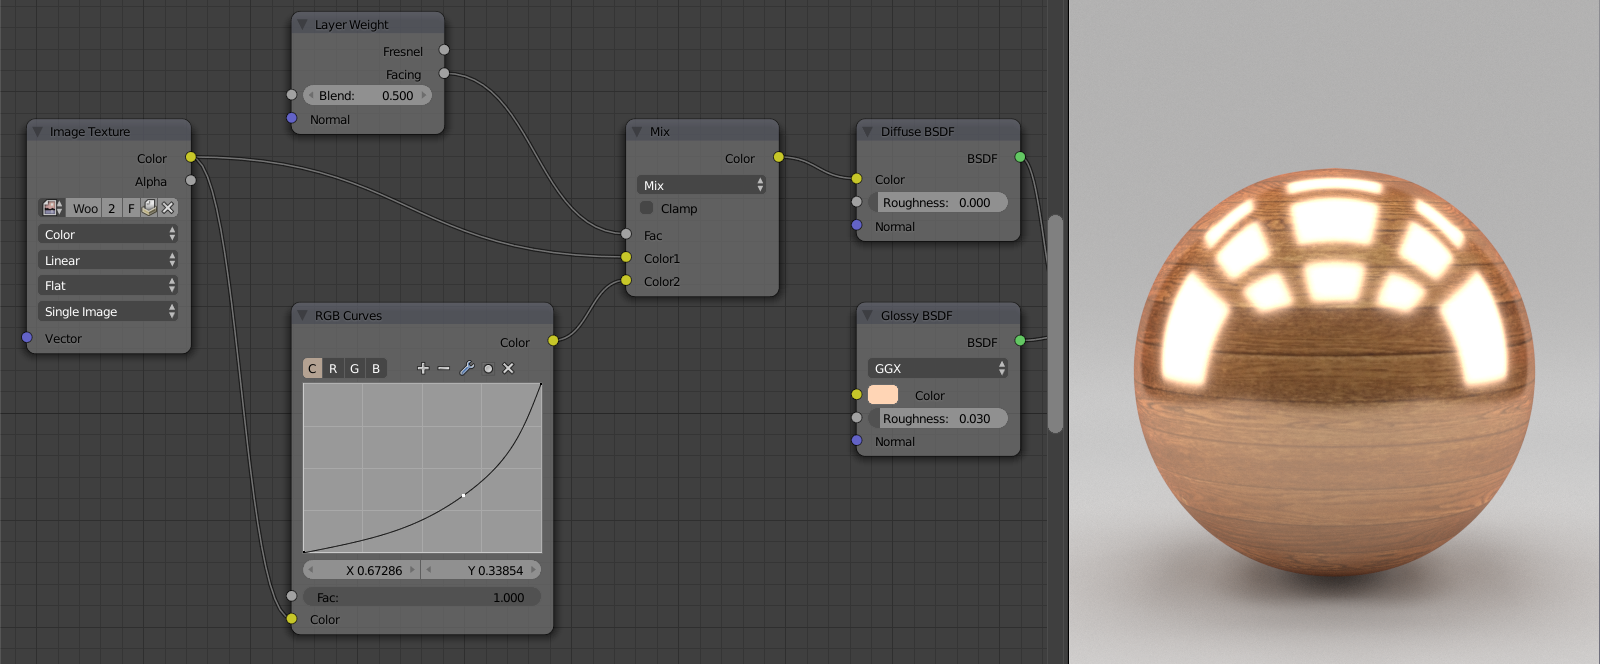
\includegraphics[scale=0.41]{step2}
\end{figure}

\newpage
\section{创建\underline{高光贴图}(Specular Map)}
高光贴图是一种基于灰度值来确定何处有光泽/高光的类型的贴图。幸运的是,在Blender里,这很容易实现。添加一个\textbf{RGB to BW}\emph{(Add>Converter>RGB to BW)}节点,并将它连接到基础图像,然后再添加一个\textbf{\underline{颜色渐变}(ColorRamp)}\emph{(Add>Converter>ColorRamp)}节点控制效果影响。

\begin{figure}[hb]
    \centering
    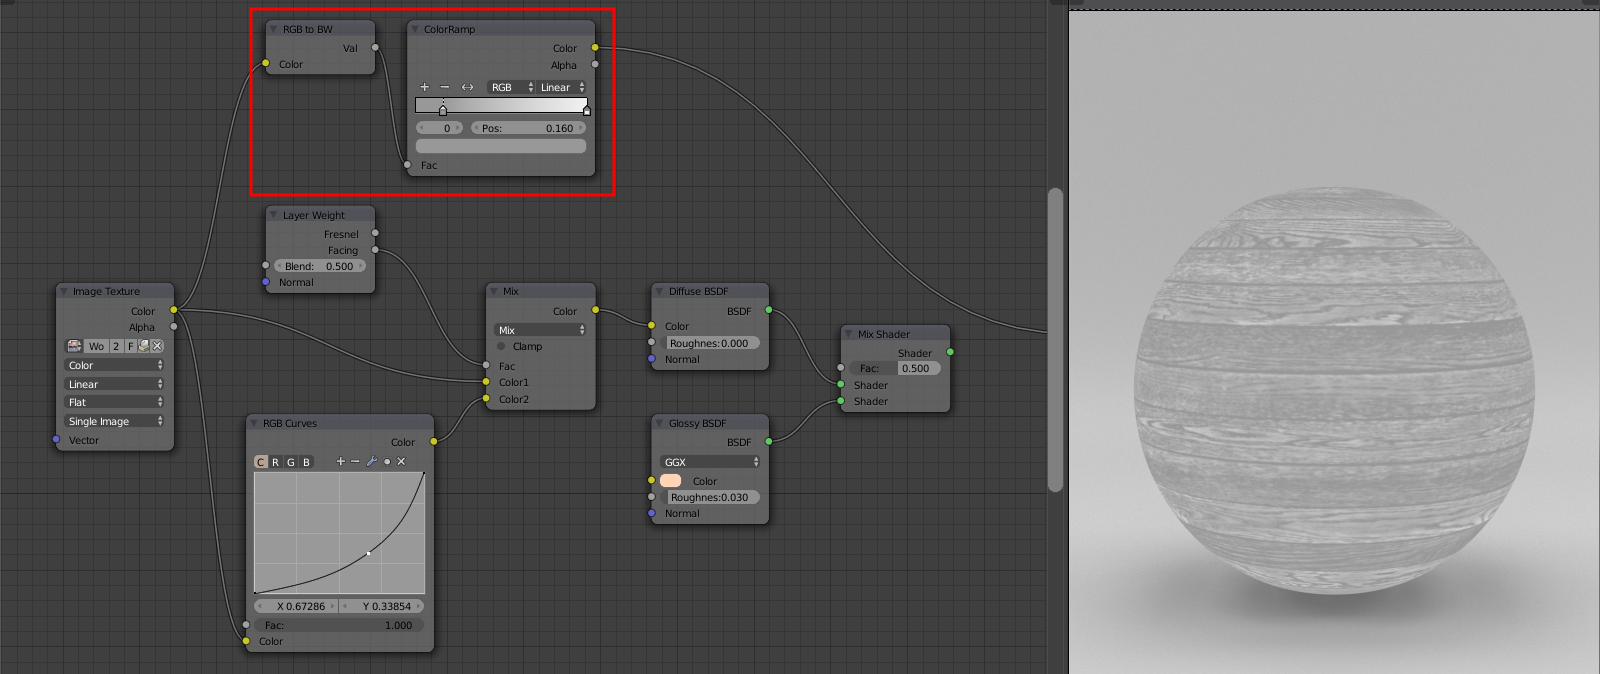
\includegraphics[scale=0.41]{step3}
\end{figure}

\section{添加\underline{基于物理的着色}(Physically-based Shading)}
在现实中,非金属/电介质物体和表面在掠射角会产生更多定义的反射\footnote{此处原文为more-defined reflections,译者水平有限,暂且翻译为“更多定义的反射”。},这也被称为菲涅耳反射率。

我们可以利用第二步中层权重节点的输出信息和第三步中创建的高光贴图,并使用\textbf{\underline{运算}(Math)}\\\emph{(Add>Converter>Math)}节点,改为\textbf{\underline{相减}(subtract)}算法,使它们的值相减。

\begin{figure}[hb]
    \centering
    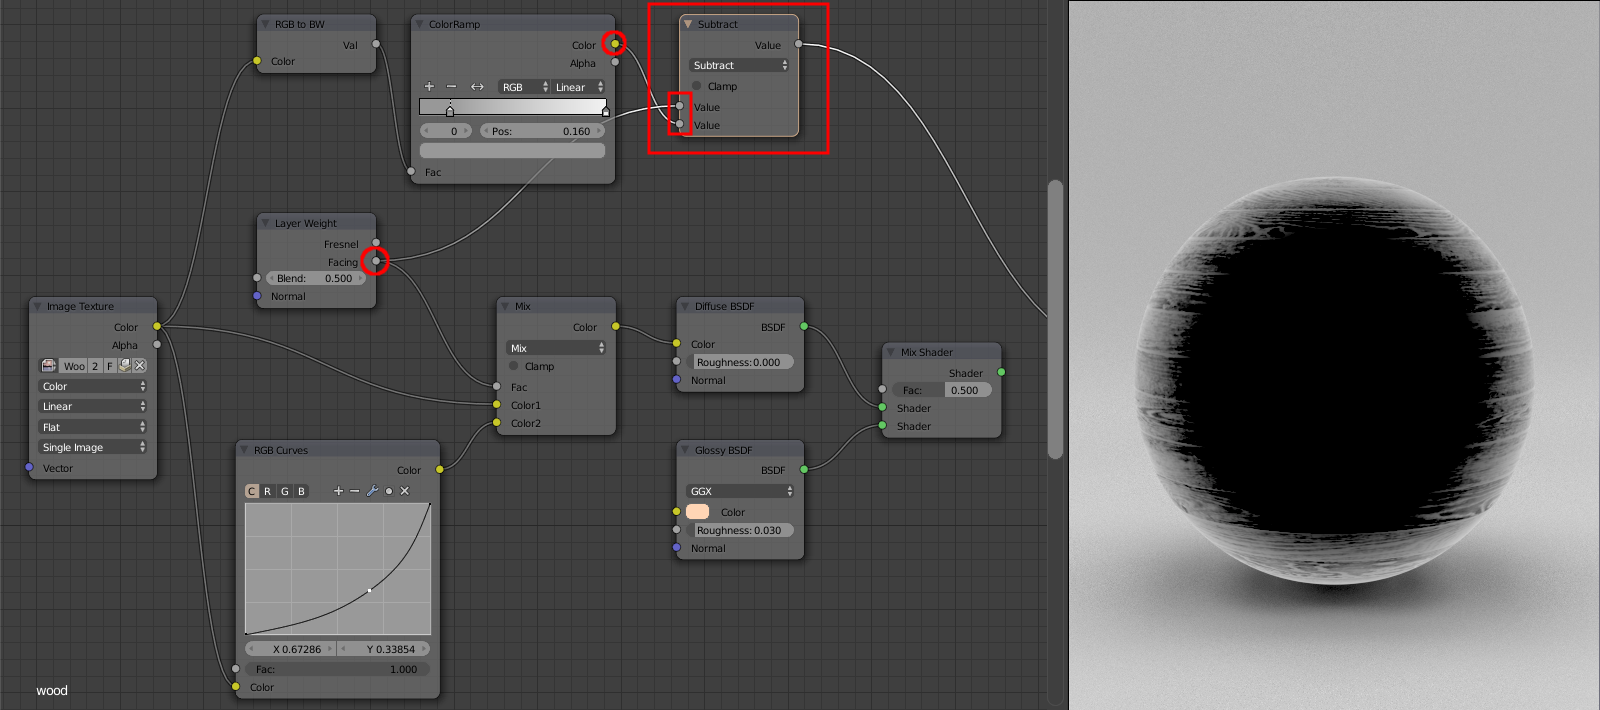
\includegraphics[scale=0.41]{step4_1}
\end{figure}

\newpage
然后我们将这个节点的输出作为混合着色器的系数输入。这一操作能产生两个结果:\textbf{\underline{菲涅耳反射率}(fresnel reflectance)}和\textbf{\underline{高光贴图}(specularity map)}。

\begin{figure}[hb]
    \centering
    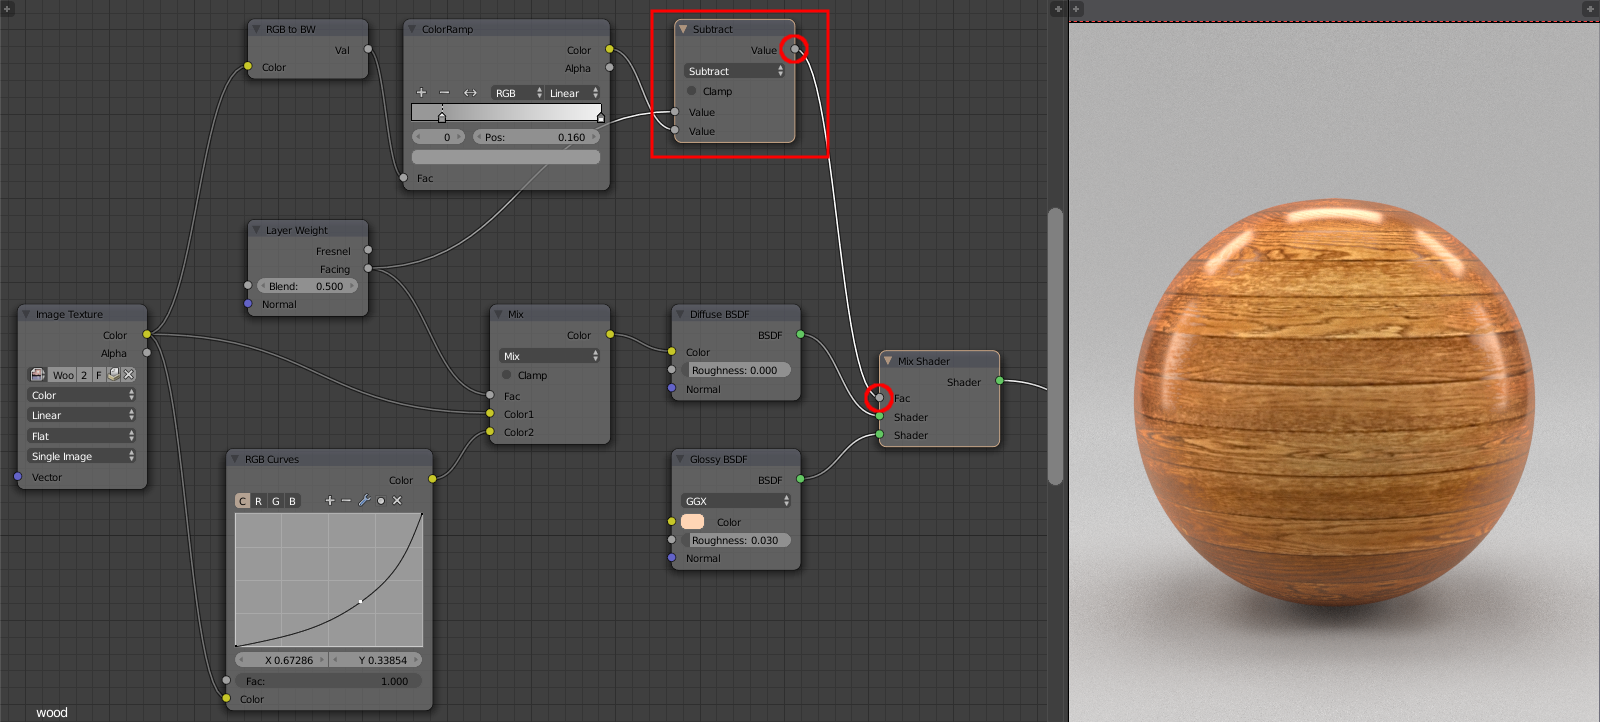
\includegraphics[scale=0.41]{step4_2}
\end{figure}

\section{创建\underline{粗糙度贴图}(Roughness Map)}
这种贴图从根本上是告诉Blender,着色器的哪部分有粗糙光泽的表面\footnote{此处原文为rough glossy surfaces,若译文不好理解的话,请看原句:This map basically tells Blender which parts of the shader has rough glossy surfaces。}。想要实现这个,我们只需简单地添加另一个\textbf{颜色渐变}节点,并把之前步骤中所使用的\textbf{GB to BWR}节点作为\textbf{系数}输入。

\begin{figure}[hb]
    \centering
    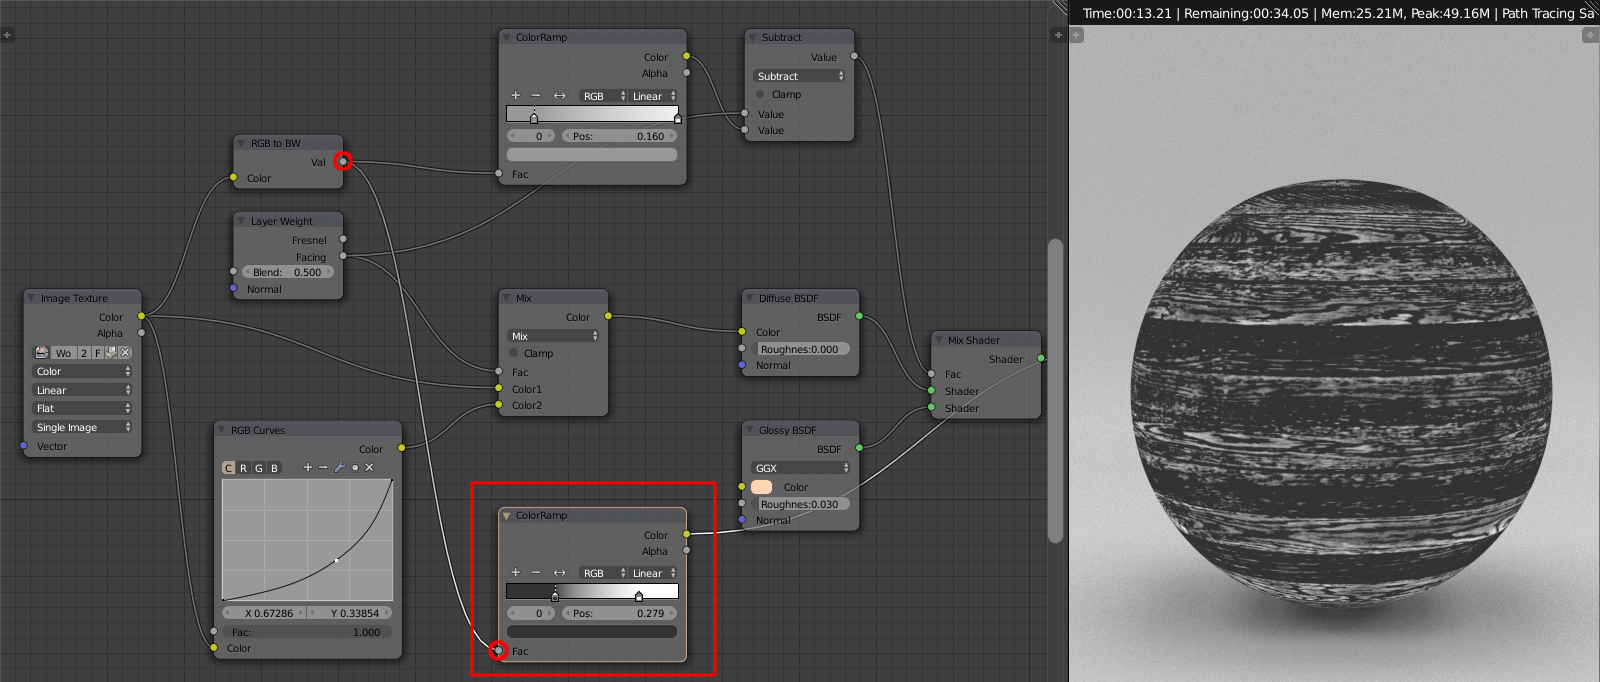
\includegraphics[scale=0.41]{step5_1.png}
\end{figure}

\newpage
将\textbf{颜色渐变}节点的颜色输出连接到\textbf{光泽BSDF}节点的\textbf{\underline{糙度}(Roughness)}输入。现在我们相当于有了一个可以轻微调整的伪粗糙度的伪装\footnote{此处原词为mask。},但是我们希望能够借用颜色渐变节点的梯度变化\footnote{此处原文为ramps,类似于节点中可以移动调整的滑条。}。

\begin{figure}[hb]
    \centering
    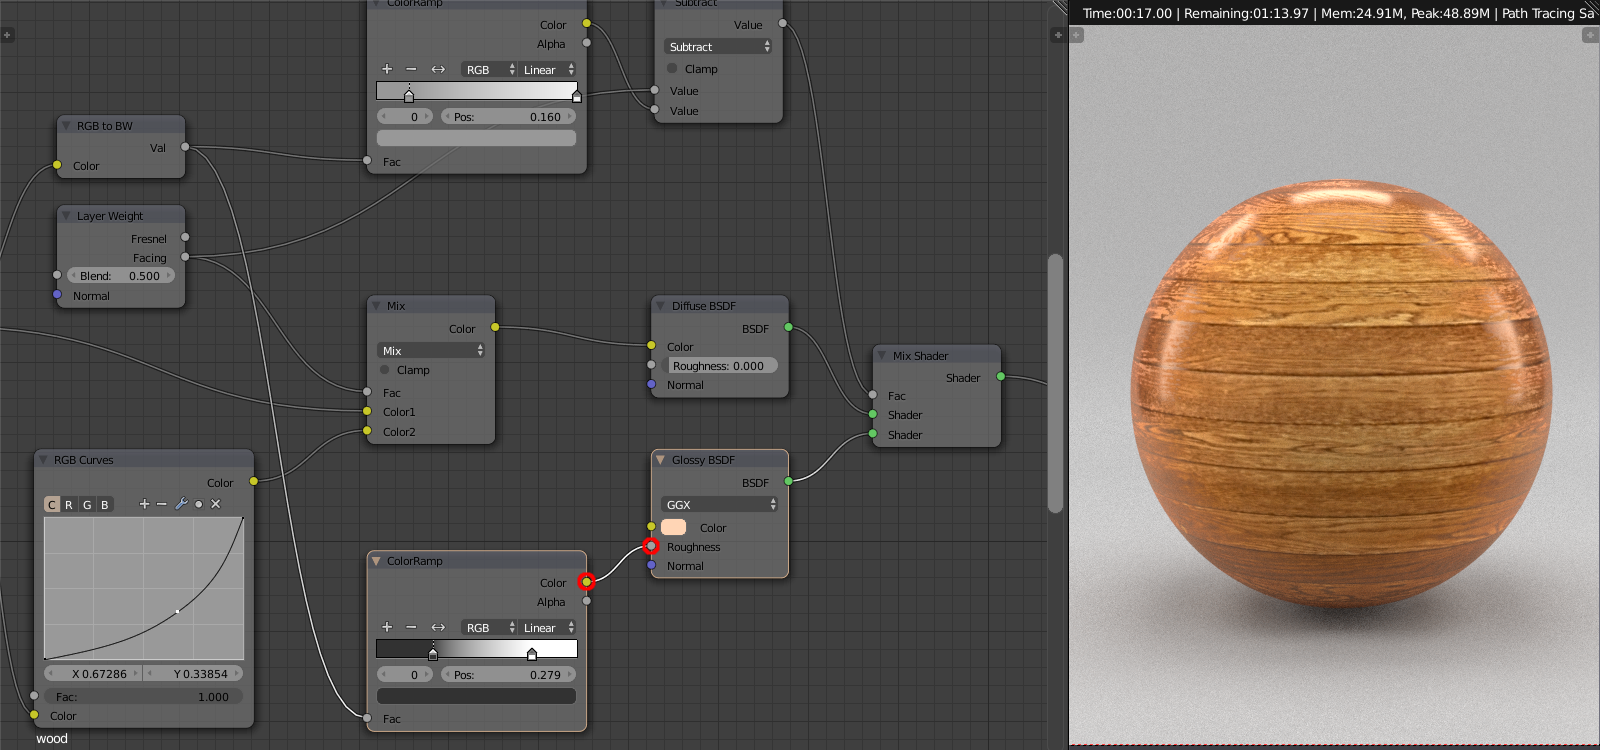
\includegraphics[scale=0.41]{step5_2.png}
\end{figure}

\section{创建\underline{法线贴图}(Normal Map)}
相较于使用专用的法线贴图时所自然得到的,它的工作原理就像一种变通方法,但其效果相对地更加接近及不可区分。

添加一个\textbf{\underline{凹凸}(Bump)}\emph{(Add>Vector>Bump)}节点,并将\textbf{RGB to BW}节点的\textbf{\underline{值}(Value)}输出连接到凹凸节点的\textbf{\underline{高度}(Height)}输入。为了能在着色器上看到效果,把凹凸节点的\textbf{\underline{法线}(Normal)}输出连接到相应着色器的\textbf{\underline{法线}(Normal)}的输入。

\begin{figure}[hb]
    \centering
    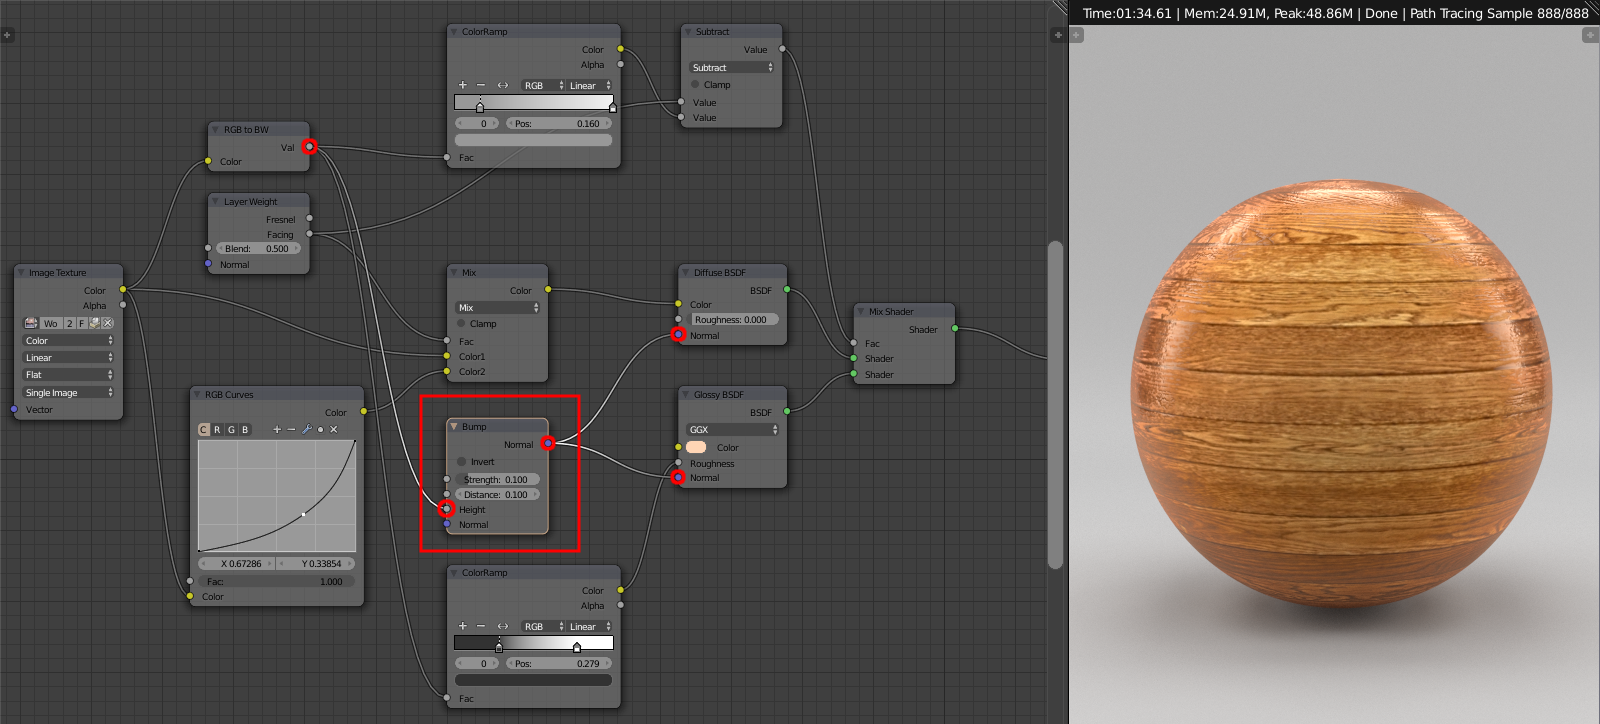
\includegraphics[scale=0.41]{step6.png}
\end{figure}

\newpage
\section{创建\underline{置换贴图}(Displacement Map)}
依据先前讨论的相同技术,我们将从中创建凹凸的材质,效果质量是在已经存在的法线贴图之上,甚至更具真实感。\footnote{若译文不好理解,请看原句:Deriving the same techniques previously discussed, we’ll be creating the material bump,
on top of the already existing normal maps, for even more realism.}

把\textbf{RGB to BW}节点的\textbf{\underline{值}(Value)}输出连接到一个\textbf{颜色渐变}节点上,并调整滑块\footnote{此处原词为sliders。},建立从纯黑到纯白的紧凑过渡。
\begin{figure}[hb]
    \centering
    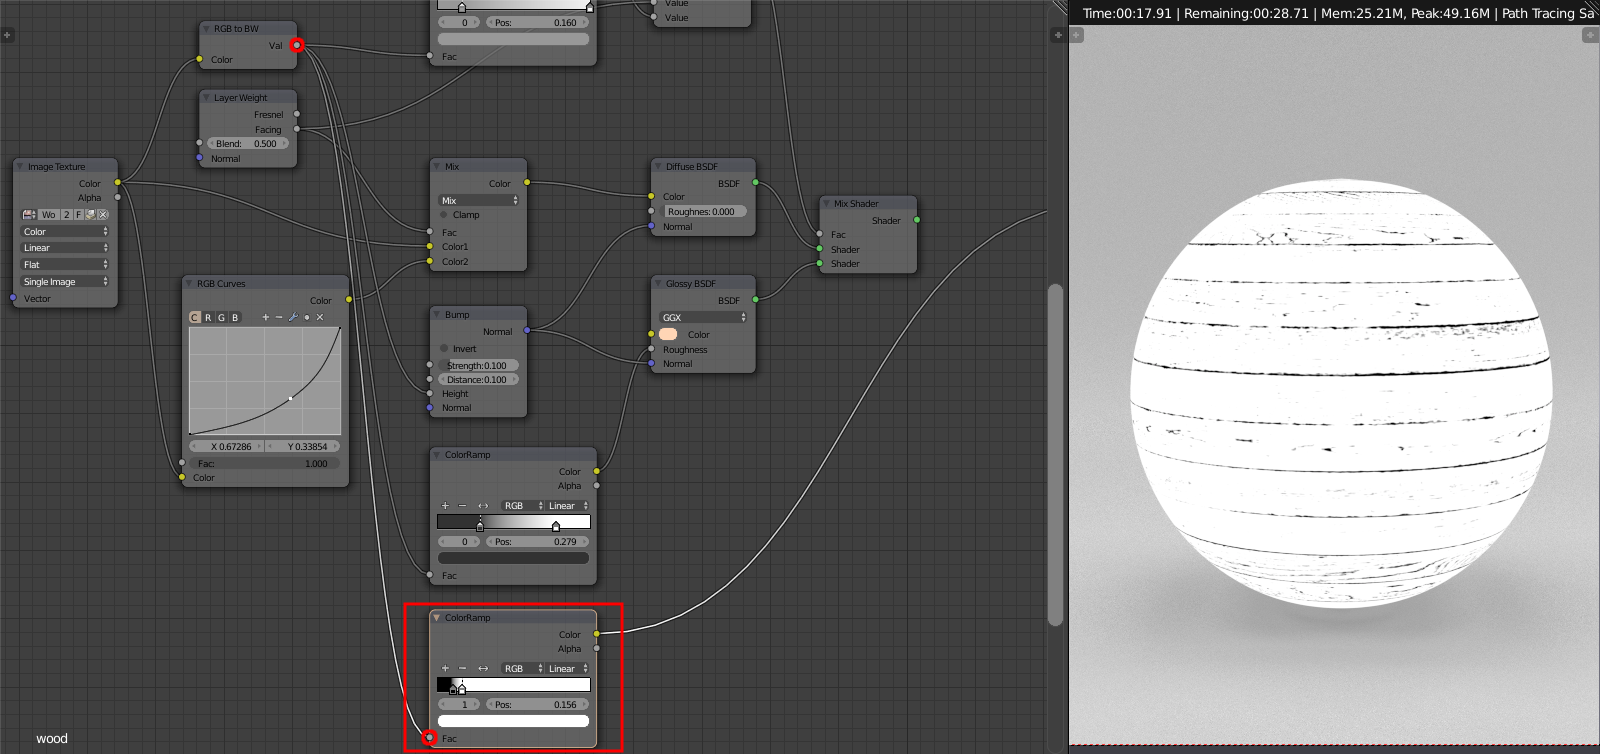
\includegraphics[scale=0.41]{step7_1.png}
\end{figure}

添加一个\textbf{运算}节点,并将其算法设置为\textbf{\underline{相乘}(Multiply)},把它连接到\textbf{\underline{输出}(Output)}节点的\textbf{\underline{置换}(Displacement)}输入。第二个滑条的值决定了此贴图映射的强度。

\begin{figure}[hb]
    \centering
    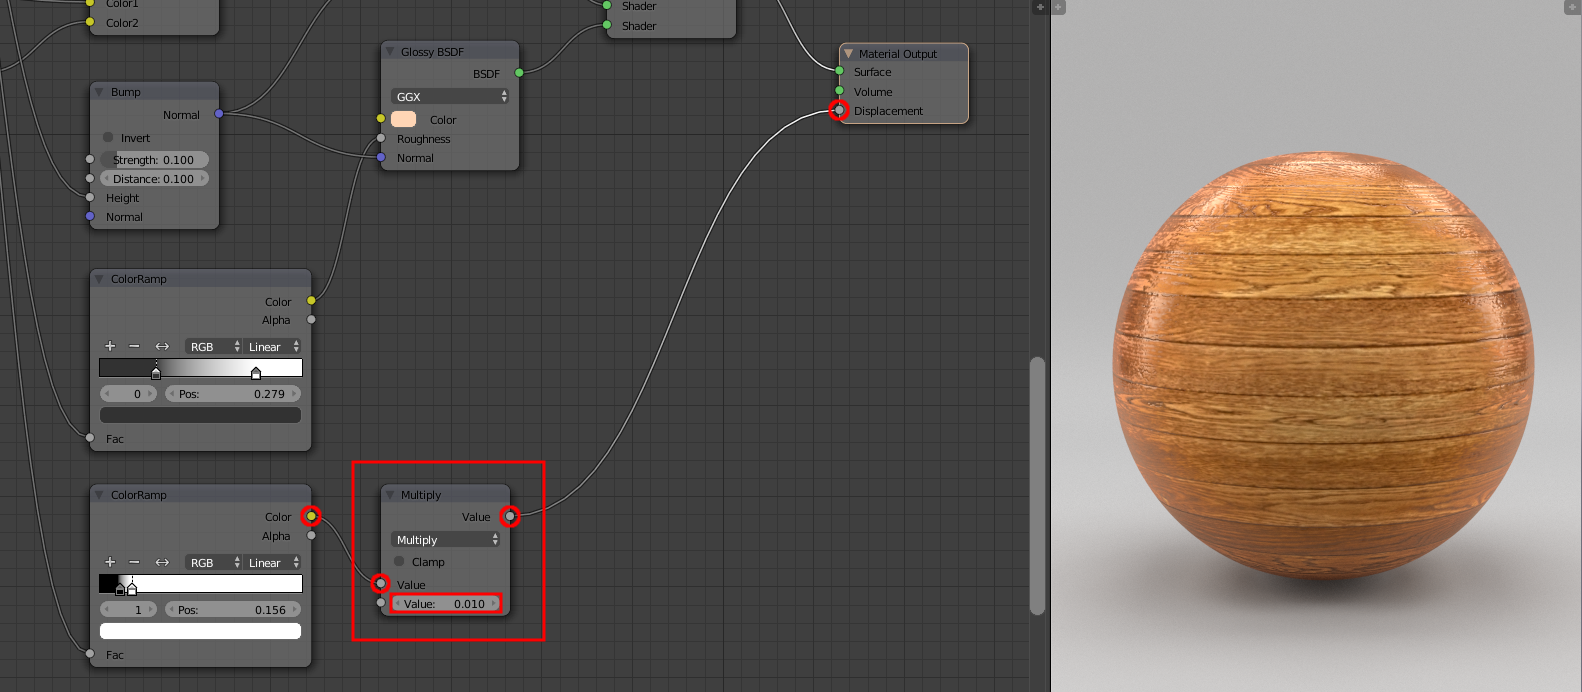
\includegraphics[scale=0.41]{step7_2.png}
\end{figure}

\newpage
\section{创建Cavity贴图}
同置换贴图结合使用,Cavity贴图\footnote{Cavity贴图本质上是一个黑白遮罩,它可以让你访问模型上的裂缝和高频细节。}能够表现在裂隙中的灰尘和尘土、\underline{遮挡}(occlusion)等诸如此类的效果。

添加一个\textbf{漫反射BSDF}节点,并将其设置接近为深灰色(或着类似的颜色),然后通过一个\textbf{混合着色器}节点将其和我们之前创建并已经存在的着色器(漫反射和光泽)一起混合。
\begin{figure}[hb]
    \centering
    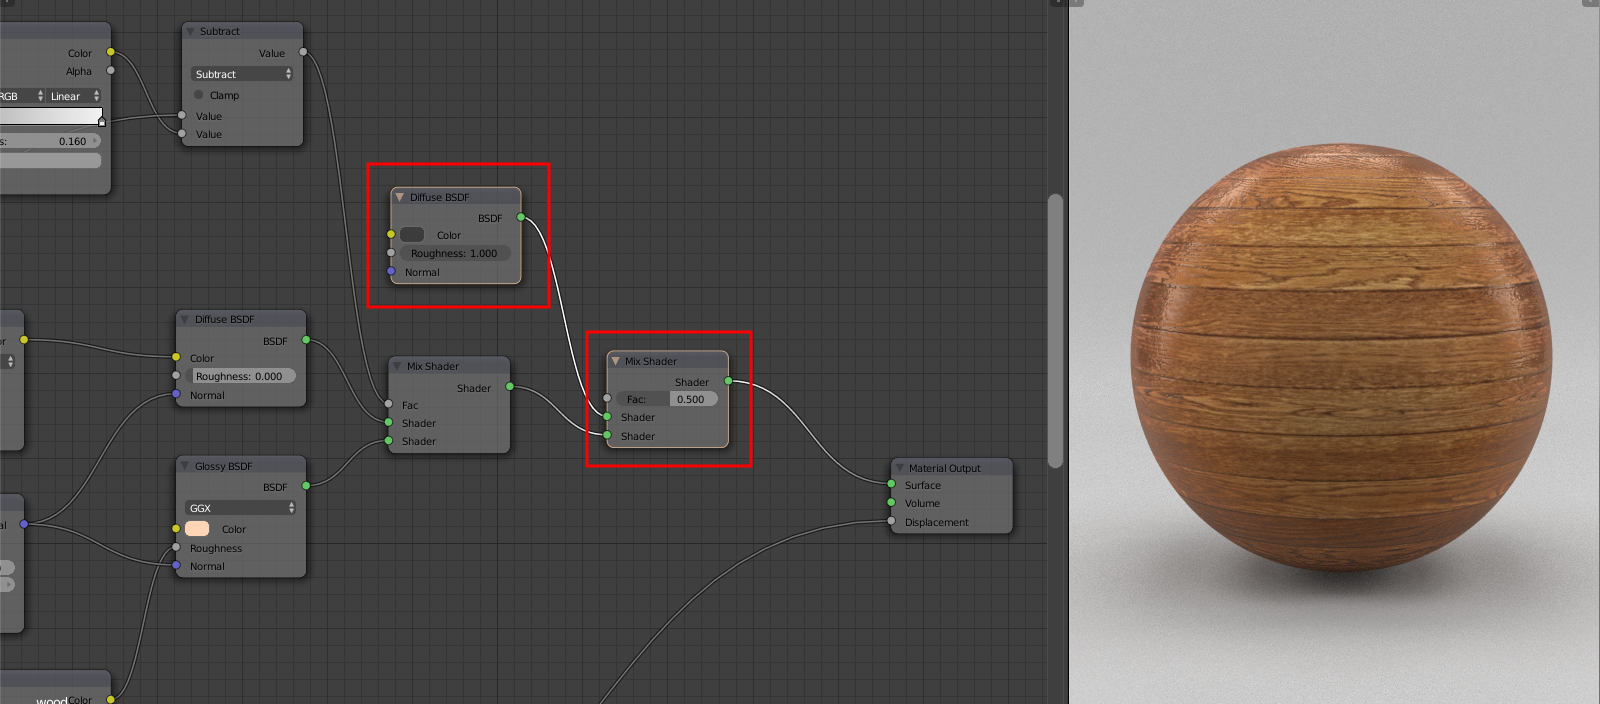
\includegraphics[scale=0.41]{step8_1.png}
\end{figure}

现在我们只是需要具体去确定哪部分是会有Cavity伪装\footnote{此处原词为masks。}。就像\textbf{第7个步骤},添加一个\textbf{颜色渐变}节点,使用浅灰色,而不是使用左边的颜色滑块来调纯黑色。
\begin{figure}[hb]
    \centering
    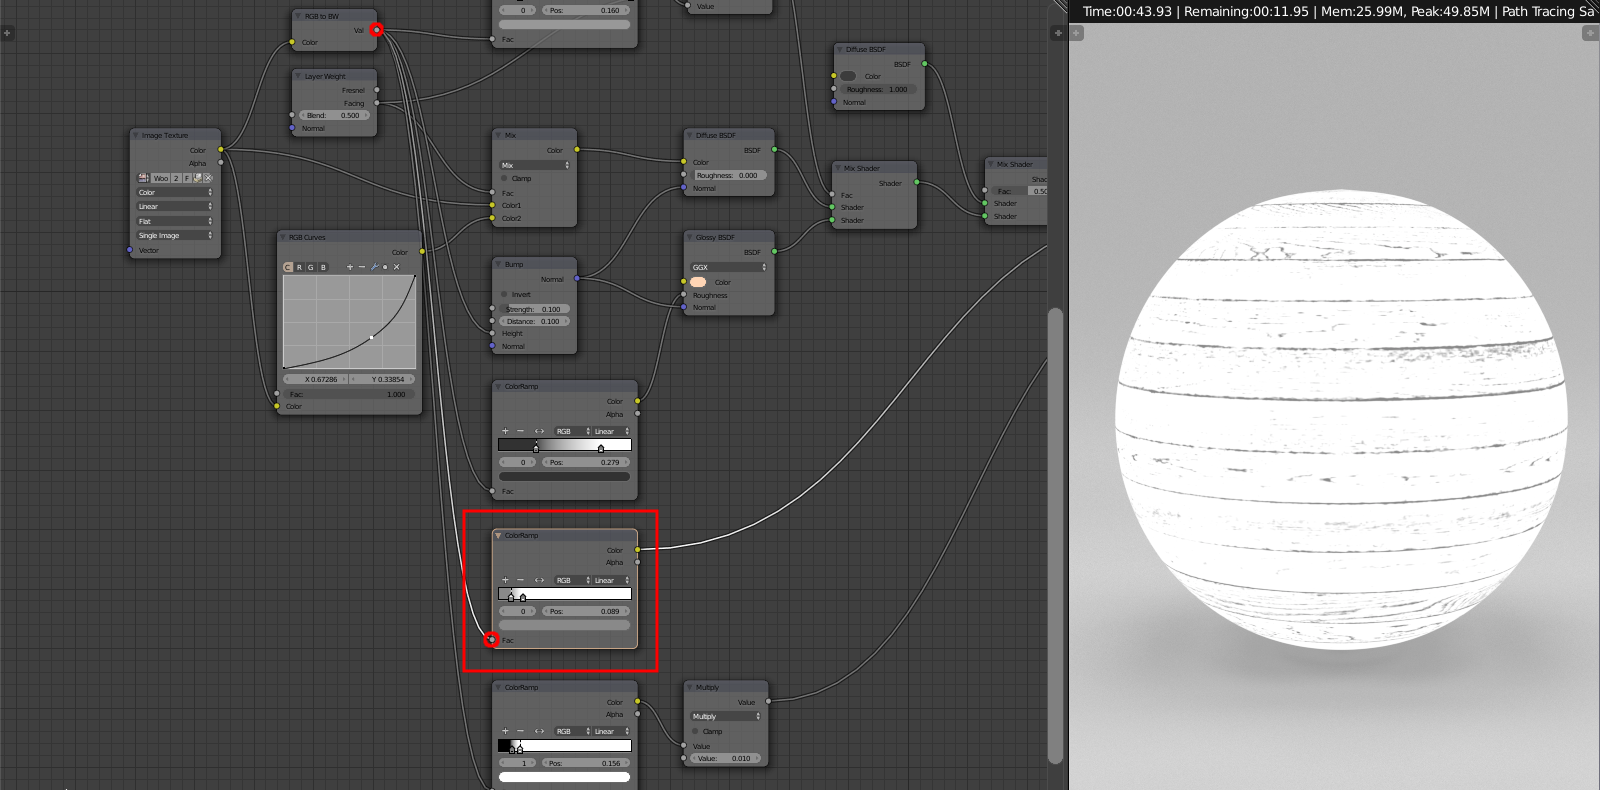
\includegraphics[scale=0.41]{step8_2.png}
\end{figure}

\newpage
最后,把\textbf{颜色渐变}节点的\textbf{颜色}输出连接到\textbf{混合着色器}的\textbf{系数}输入。
\begin{figure}[hb]
    \centering
    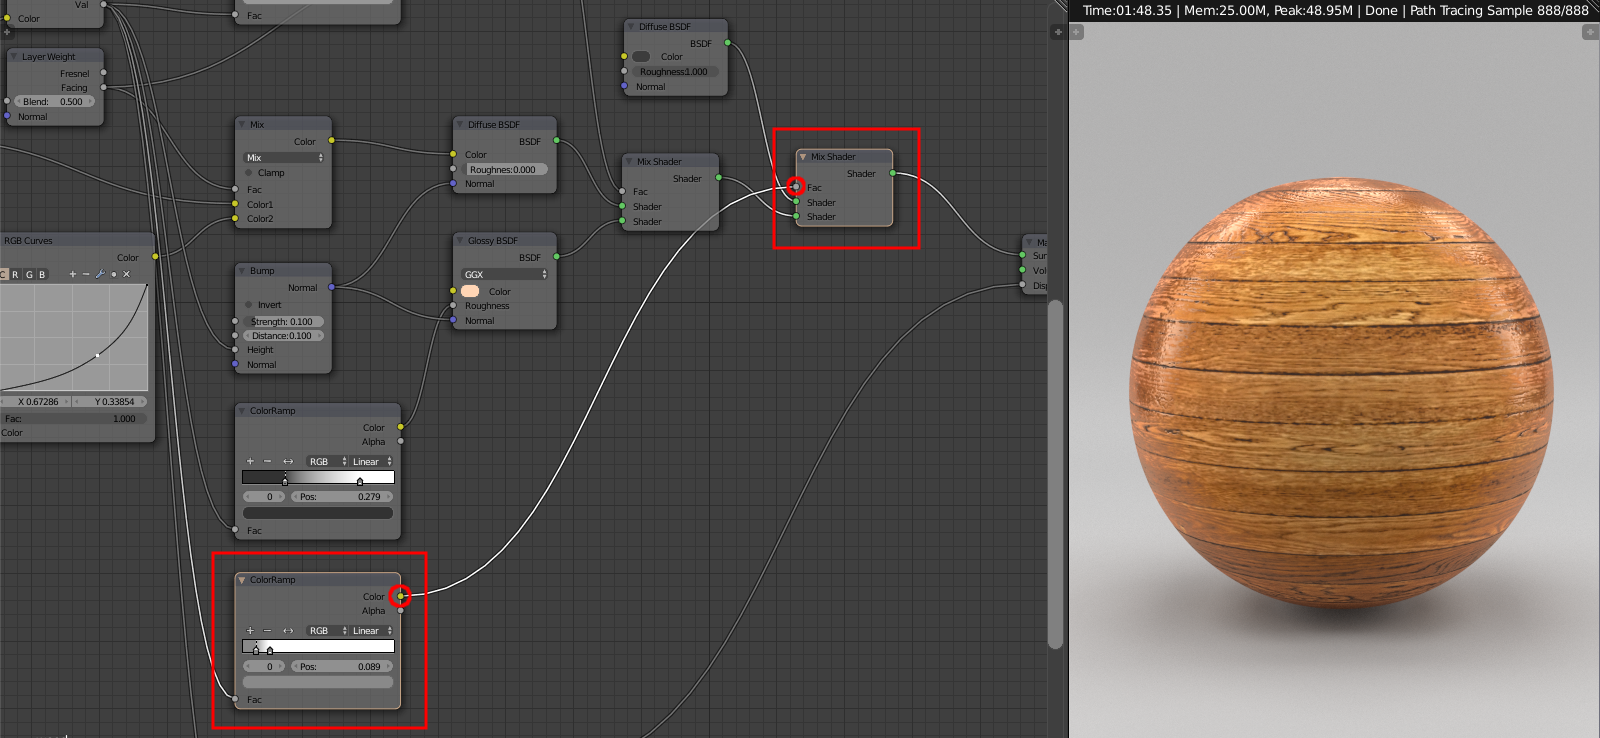
\includegraphics[scale=0.41]{step8_3.png}
\end{figure}

\noindent {\large\textbf{结语}}

这里所展示的技巧、步骤和变通方法只是在关于如何使用节点创建贴图的方面上触及到很表层的知识。同其它的效果一同使用,如\underline{划痕}(scratches)、\underline{表面灰尘}(surface dusts)等类似的,这将会是你艺术工作流上的一大增强手段。

我强烈建议你去进一步探索,打破我所展示的方法,并最终找到更直观和更有效的方法。

\noindent \rule[4pt]{500pt}{.5pt}

如果你喜欢这篇文章的话,那就留下评论,并把它分享给你的朋友吧!

想关注我的话,可以通过以下连接:
\begin{itemize}
    \item \href{http://www.reynantemartinez.com/}{网站}
    \item \href{https://www.facebook.com/artofreynantemartinez}{脸书}
    \item \href{https://twitter.com/reynantem}{推特}
\end{itemize}

祝使用Blender愉快!

- Reyn
\end{document}